\documentclass[../report.tex]{subfiles}

\begin{document}
\subsection{Giới thiệu về ngắt}
Ngắt (Interrupt) - là một số sự kiện khẩn cấp bên trong hoặc bên ngoài bộ vi điều khiển xảy ra, 
buộc vi điều khiển tạm dừng thực hiện chương trình hiện tại, 
phục vụ ngay lập tức nhiệm vụ mà ngắt yêu cầu – nhiệm vụ này gọi là trình phục vụ ngắt (ISR: Interrupt Service Routine).

Phân biệt ngắt với hỏi vòng: 
\begin{itemize}
\item Trong phương pháp sử dụng ngắt: mỗi khi có một thiết bị bất kỳ cần 
được phục vụ thì nó báo cho bộ vi điều khiển bằng cách gửi một tín hiệu ngắt. 
Khi nhận được tín hiệu ngắt thì bộ vi điều khiển ngừng tất cả những gì nó 
đang thực hiện để chuyển sang phục vụ thiết bị gọi ngắt. 
Chương trình ngắt được gọi là trình phục vụ ngắt ISR (Interrupt Service Routine) 
hay còn gọi là trình quản lý ngắt (Interrupt Handler). 
Sau khi phục vụ ngắt xong, bộ vi xử lý lại quay trở lại 
điểm bị ngắt trước đó và tiếp tục thực hiện công việc.

\item Trong phương pháp thăm dò: bộ vi điều khiển kiểm tra liên tục tình trạng của tất cả các thiết bị, 
nếu thiết bị nào có yêu cầu thì nó dừng lại phục vụ thiết bị đó. 
Sau đó nó tiếp tục kiểm tra tình trạng của thiết bị kế tiếp cho đến hết. 
Phương pháp thăm dò rất đơn giản, nhưng nó lại rất lãng phí thời gian để kiểm tra các 
thiết bị kể cả khi thiết bị đó không cần phục vụ. 
Trong trường hợp có quá nhiều thiết bị thì phương án thăm dò tỏ ra không hiệu quả, 
gây ra chậm trễ cho các thiết bị cần phục vụ.
\end{itemize}

\subsection{Các ngắt trong 8051}
Thực tế chỉ có 5 ngắt dành cho người dùng trong 8051 nhưng các 
nhà sản xuất nói rằng có 6 ngắt vì họ tính cả lệnh RESET. 
Sáu ngắt của 8051 được phân bố như sau:
\begin{itemize}
\item RESET: Khi chân RESET được kích hoạt từ 8051, bộ đếm chương trình nhảy về địa chỉ 0000H.  Đây là địa chỉ bật lại nguồn.
\item 2 ngắt dành cho các bộ định thời: 1 cho Timer0 và 1 cho Timer1. Địa chỉ tương ứng của các ngắt này là 000BH và 001BH.
\item 2 ngắt dành cho các ngắt phần cứng bên ngoài: chân 12 (P3.2) và 13 (P3.3) của cổng P3 là các ngắt phần cứng bên ngoài INT0 và INT1 tương ứng. Địa chỉ tương ứng của các ngắt ngoài này là 0003H và 0013H.
\item Truyền thông nối tiếp: có 1 ngắt chung cho cả nhận và truyền dữ liệu nối tiếp. Địa chỉ của ngắt này trong bảng vector ngắt là 0023H.
\end{itemize}

\subsection{Các trình phục vụ ngắt 8051}
Đối với mỗi ngắt thì phải có một trình phục vụ ngắt (ISR) 
hay trình quản lý ngắt để đưa ra nhiệm vụ cho bộ vi điều khiển khi được gọi ngắt. 
Khi một ngắt được gọi thì bộ vi điều khiển sẽ chạy trình phục vụ ngắt. 
Đối với mỗi ngắt thì có một vị trí cố định trong bộ nhớ để giữ địa chỉ ISR của nó. 
Nhóm vị trí bộ nhớ được dành riêng để lưu giữ địa chỉ của các ISR được gọi là bảng vector ngắt.
\begin{table}[H]
\centering
\begin{tabular}{|l|c|c|c|}
\hline 
\textbf{Ngắt} & \textbf{Cờ ngắt} & \textbf{Địa chỉ trình phục vụ ngắt} & \textbf{Số thứ tự ngắt} \\
\hline
Reset & - & 0000h & - \\
\hline
Ngắt ngoài 0 & IE0 & 0003h & 0 \\
\hline
Timer 0 & TF0 & 000Bh & 1 \\
\hline
Ngắt ngoài 1 & IE1 & 0013h & 2 \\
\hline
Timer 1 & TF1 & 001Bh & 3 \\
\hline
Ngắt truyền thông & RI/TI & 0023h & 4 \\
\hline
\end{tabular}
\caption{Bảng vector ngắt của 8051}
\end{table}

Trong lập trình C trên Keil C cho 8051, chúng ta khai báo trình phục vụ ngắt bằng cách thêm interrupt X 
vào sau khai báo hàm (X là số thứ tự ngắt). 

\subsection{Cho phép và cấm ngắt trong 8051}
Khi bật lại nguồn thì tất cả mọi ngắt đều bị cấm (bị che), 
có nghĩa là không có ngắt nào được bộ vi điều khiển đáp ứng trừ khi chúng được kích hoạt.

Các ngắt phải được kích hoạt bằng phần mềm để bộ vi điều khiển đáp ứng chúng. 
Có một thanh ghi được gọi là thanh ghi cho phép ngắt \textbf{IE} (Interrupt Enable) – 
ở địa chỉ A8h chịu trách nhiệm về việc cho phép và cấm các ngắt.

\begin{table}[H]
\centering
\begin{tabular}{|c|c|c|l|}
\hline
\textbf{Bit} & \textbf{Tên} & \textbf{Địa chỉ} & \textbf{Chức năng} \\
\hline
7 & EA & AFh & Cho phép/cấm hoạt động của cả thanh ghi.  \\
\hline
6 & - & AEh & Chưa sử dụng.  \\
\hline
5 & - & ADh & Chưa sử dụng. \\
\hline
4 & ES & ACh & Cho phép ngắt cổng truyền thông nối tiếp. \\
\hline
3 & ET1 & ABh & Cho phép ngắt Timer 1. \\
\hline
2 & EX1 & AAh & Cho phép ngắt ngoài 1. \\
\hline
1 & ET0 & A9h & Cho phép ngắt Timer 0. \\
\hline
0 & EX0 & A8h & Cho phép ngắt ngoài 0. \\ 
\hline
\end{tabular}
\caption{Thanh ghi cho phép ngắt \textbf{IE}}
\end{table}
\subsection{Mức độ ưu tiên các ngắt trong 8051}
Mỗi ngắt có 2 chế độ ưu tiên: 0 hoặc 1. Được thiết lập nhờ thanh ghi IP. 
\begin{figure}[H]
\centering
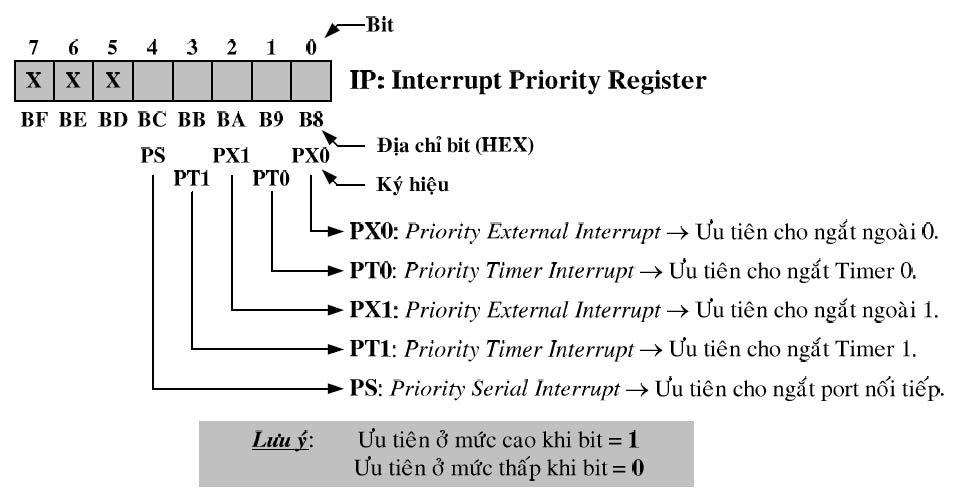
\includegraphics[width=12cm]{figures/ip-register.jpg}
\end{figure}

\subsection{Ngắt timer trong 8051}
Có 2 ngắt timer trong 8051 là timer 0 và timer 1 với chức năng giống nhau. 
Các ngắt timer được thiết lập chế độ hoạt động bằng thanh ghi TMOD.

\begin{table}[H]
\centering
\begin{tabular}{|c|c|l|}
\hline
\textbf{Bit} & \textbf{Tên} & \textbf{Chức năng} \\
\hline
7 & Gate & - \\
\hline
6 & C/T & 1 nếu như sử dụng timer/counter 1 làm counter, 0 nếu như sử dụng làm timer. \\
\hline
5 & M1 & Bit cao thiết lập chế độ cho timer/counter 1.  \\
\hline
4 & M0 & Bit thấp thiết lập chế độ cho timer/counter 1.  \\
\hline
3 & Gate & - \\
\hline
2 & C/T & 1 nếu như sử dụng timer/counter 0 làm counter, 0 nếu như sử dụng làm timer. \\
\hline
1 & M1 & Bit cao thiết lập chế độ cho timer/counter 0.  \\
\hline
0 & M0 & Bit thấp thiết lập chế độ cho timer/counter 0.  \\
\hline

\end{tabular}
\caption{Các bit trong thanh ghi TMOD (Timer Mode Control)}
\end{table}

\begin{table}[H]
\centering
\begin{tabular}{|c|c|c|l|}
\hline
\textbf{M1} & \textbf{M0} & \textbf{Chế độ} & \textbf{Mô tả}    \\
\hline
0 & 0 & 0 & Sử dụng thanh ghi TH làm bộ đếm 8 bit và thanh ghi TL làm bộ đếm 5 bit \\
\hline
0 & 1 & 1 & Sử dụng thanh ghi TH làm bộ đếm 8 bit và thanh ghi TL làm bộ đếm 8 bit \\
\hline
1 & 0 & 2 & Sử dụng chỉ thanh ghi TL làm bộ đếm 8 bit \\
\hline
1 & 1 & 3 & Timer 0 trong chế độ 3 trở thành 2 bộ đếm 8 bit tách biệt.  \\
& & & Timer 1 vẫn có thể được sử dụng nhưng không tạo ra tín hiệu ngắt \\
\hline
\end{tabular}
\caption{Các chế độ của timer/counter} 
\end{table}

\begin{table}[H]
\centering
\begin{tabular}{|c|c|l|}
\hline
\textbf{Bit} & \textbf{Kí hiệu} & \textbf{Chức năng}  \\
\hline
7 & TF1 & Cờ tràn của timer 1. Được xóa khi ngắt tương ứng được thực thi. \\
\hline
6 & TR1 & Điều khiển timer 1. Gán bằng 1 để bắt đầu đếm.  \\
\hline
5 & TF0 & Cờ tràn của timer 0. Được xóa khi ngắt tương ứng được thực thi. \\
\hline
4 & TR0 & Điều khiển timer 0. Gán bằng 1 để bắt đầu đếm. \\
\hline
3 & IE1 &  \\
\hline
2 & IT1 & Gán bằng 1 nếu timer 1 tích cực sườn âm, bằng 0 nếu tích cực mức thấp. \\
\hline
1 & IE0 & \\
\hline
0 & IT0 & Gán bằng 0 nếu timer 1 tích cực sườn âm, bằng 0 nếu tích cực mức thấp. \\
\hline
\end{tabular}
\caption{Thanh ghi TCON (Timer Control)} 
\end{table}

Trong bài này chỉ sử dụng để làm timer (không sử dụng để làm counter) nên C/T = 0. 
Đồng thời 2 timer đều sử dụng ở chế độ 16 bit nên M1 = 0 và M0 = 1. 
Hai thanh ghi TH, TL là 2 thanh ghi lưu trữ giá trị đếm của timer. Khi giá trị này bị tràn thì cờ TF được set và 
tín hiệu ngắt được sinh ra.  

Bộ đếm timer sẽ hoạt động với tần số bằng $1/12$ tần số của bộ dao động thạch anh. 

\end{document}
